\documentclass[table]{beamer}
%%\documentclass[handout]{beamer}

\mode<presentation>
{
  \definecolor{navitialight}{RGB}{126,186,200}
  \definecolor{navitiadark}{RGB}{76,102,114}

  \useoutertheme[subsection=false]{miniframes}
  %%\useoutertheme[footline=authortitle]{miniframes}
  \usecolortheme[named=navitiadark]{structure}
  %%\usecolortheme{dolphin}
  \usecolortheme{orchid}
  \useinnertheme{circles}
  \setbeamerfont{block title}{size=\normalsize}
  \setbeamercovered{transparent}

  %%% le foot pour avoir la numérotation des slides %%%
  \setbeamertemplate{footline}{%
    \leavevmode%
    \hbox{%
      \begin{beamercolorbox}[wd=.5\paperwidth,ht=2.5ex,dp=1.125ex,
        leftskip=.3cm plus1fill,rightskip=.3cm]{author in head/foot}%
        \usebeamerfont{title in head/foot}\insertshorttitle
      \end{beamercolorbox}%
      \begin{beamercolorbox}[wd=.5\paperwidth,ht=2.5ex,dp=1.125ex,
        leftskip=.3cm,rightskip=.3cm plus1fil]{title in head/foot}%
        \usebeamerfont{author in head/foot}\insertshortauthor\hfill
        \insertframenumber/\inserttotalframenumber
      \end{beamercolorbox}%
    }%
    \vskip0pt%
  }

  \setbeamercolor{palette primary}{fg=white,bg=navitiadark}
  \setbeamercolor{palette secondary}{fg=white,bg=navitialight}
  \setbeamercolor{palette tertiary}{fg=white,bg=navitiadark}
  \setbeamercolor{palette quaternary}{fg=white,bg=navitialight}
}

\mode<handout>
{
  \usepackage{pgfpages}
  \pgfpagesuselayout{4 on 1}[a4paper,border shrink=5mm,landscape]
}

\usepackage[utf8]{inputenc}
\usepackage{lmodern}
\usepackage[T1]{fontenc}
\usepackage[english,francais]{babel}
\usepackage{multirow}
\usepackage{hhline}

\newcommand{\nologo}{\setbeamertemplate{logo}{}}

\newenvironment{foreignpar}[1][english]{%
    \em\selectlanguage{#1}%
}{}
\newcommand*{\foreign}[2][english]{%
    \emph{\foreignlanguage{#1}{#2}}%
}

\title{Transport Optimisé À la Demande}

\author{L'équipe TOÀD}
%%\author{Vincent Chabot \and Romain Choquet \and Guillaume Pinot \and Pascal Rhod}

\institute[Kisio Digital] % (optional, but mostly needed)
{
  Kisio Digital\\
  20 rue Hector Malot\\
  75012 Paris, France}
%% - Use the \inst command only if there are several affiliations.
%% - Keep it simple, no one is interested in your street address.

\date{Soutenance SWAT 2017}
%% - Either use conference name or its abbreviation.
%% - Not really informative to the audience, more for people (including
%%   yourself) who are reading the slides online

%% If you have a file called "university-logo-filename.xxx", where xxx
%% is a graphic format that can be processed by latex or pdflatex,
%% resp., then you can add a logo as follows:
%\pgfdeclareimage[width=.2\linewidth]{logo}{images/logo_nio}
%\logo{\pgfuseimage{logo}\hspace{.04\linewidth}}


%% Delete this, if you do not want the table of contents to pop up at
%% the beginning of each subsection:
% \AtBeginSection[]
% {
%   \begin{frame}<beamer>
%     \frametitle{Table des matières}
%     \tableofcontents[currentsection,hideothersubsections]
%   \end{frame}
% }
% \AtBeginSubsection[]
% {
%   \begin{frame}<beamer>
%     \frametitle{Table des matières}
%     \tableofcontents[currentsection,subsectionstyle=show/shaded/hide]
%   \end{frame}
% }


\begin{document}

\begin{frame}
  \titlepage
\end{frame}

\section{Problématique}

\begin{frame}{Problématique}
  Problème du transport en commun en demande faible (zone peu dense,
  heures creuses, service de nuit):
  \begin{itemize}
  \item mauvais service pour le voyageur
  \item coût élevé pour le transporteur
  \end{itemize}

  \vfill

  \begin{em}
    «~46\% des français en zone rurale se jugent loin de tout. Il faut
    travailler sur ces zones, notamment avec la mobilité partagée~»
  \end{em}

  \raggedleft --- Hervé~Richard, directeur du programme\\
  «~porte-à-porte~» SNCF
\end{frame}

\begin{frame}{La solution}
  Transport Optimisé À la Demande

  \begin{center}
    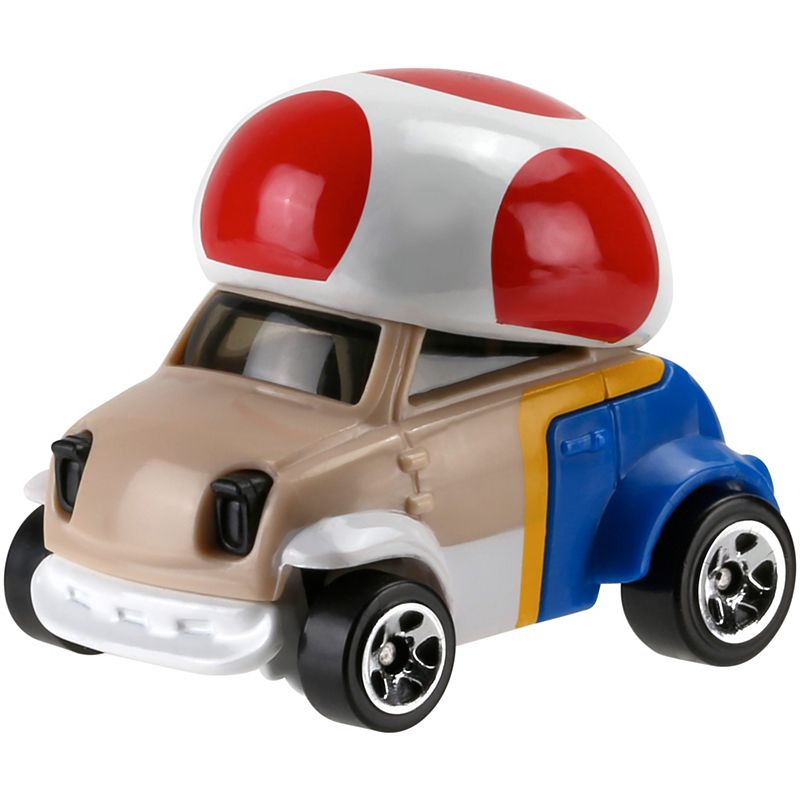
\includegraphics[width=0.4\linewidth]{images/toad}

    \emph{Responsive locomotion}
  \end{center}
\end{frame}

\begin{frame}{Le principe}
  Les réservations sont intégrées en prenant une marge de temps pour
  \begin{itemize}
  \item prendre en compte les futurs réservations
  \item s'adapter en temps réel à la réalité du terrain
  \end{itemize}
\end{frame}

\section{Simulation}

\begin{frame}{Vision voyageur}

  \begin{itemize}[<+->]
  \item Alice veut aller du 20 rue Hector Malot à la Tour Eiffel, elle
    le saisie dans l'interface. Il est 03h37.
  \item L'IHM lui propose de monter dans le transport au 44 boulevard
    Diderot à 03h45, et qu'elle arrivera au 3 avenue de Suffren avant
    04h45.
  \item Alice accepte la proposition, elle est à l'heure au point de
    rendez-vous.
  \item Le véhicule arrive à 03h52. Bob est déjà dans le véhicule.
  \item À 04h18, Bob descend 108 boulevard de Grenelle.
  \item À 04h20, Cunégonde monte au 129 boulevard de Grenelle.
  \item Alice descend à 04h31 au 3 avenue de Suffren.
  \end{itemize}
\end{frame}

\begin{frame}[allowframebreaks]{Vision conducteur}
  À 04h06, Alice et Bob sont dans le véhicule:
  \begin{itemize}
  \item 04h18, 108 boulevard Grenelle, Bob descend
  \item 04h25, 3 avenue de Suffren, Alice descend
  \end{itemize}\framebreak

  À 04h07, Cunégonde fait sa réservation:
  \begin{itemize}
  \item 04h18, 108 boulevard Grenelle, Bob descend
  \item \textbf{04h20, 129 boulevard de Grenelle, Cunégonde monte}
  \item 04h25\textbf{+6,} 3 avenue de Suffren, Alice descend
  \item \textbf{05h14, 3 Avenue Gambetta, Cunégonde descend}
  \end{itemize}
\end{frame}

\section{Une opportunité pour Keolis}

\begin{frame}{Une opportunité pour Keolis}

  \begin{itemize}
  \item gain d'image
  \item amélioration de service pour l'usager
  \item compétitivité vis à vis de son AO
  \item maîtrise complète de la solution
  \item amélioration de la connaissance des usages
  \end{itemize}
\end{frame}

\section{La concurrence}

\begin{frame}{La concurrence}

  \begin{description}
  \item[uberPOOL] solution orthogonale sur le
    modèle classique VTC
  \item[Citymapper Smartbus] flotte propre
  \item[padam] après un essai avec sa propre flotte, revente de la
    solution logicielle
  \item[bestmile] spécialisé véhicule autonome
  \item[LeCab Plus] zone à forte demande, dépendance en un tiers
  \end{description}
\end{frame}

\section{Business Model}

\begin{frame}{Business Model}
  \begin{itemize}
  \item modèle SAAS tout comme le modèle Kisio Digital
  \item projet éligible au crédit impôt recherche
  \end{itemize}
\end{frame}

\section{Réalisation}

\begin{frame}{Roadmap}
  Avant le SWAT:
  \begin{itemize}
  \item prise de contact avec des filiales pour avoir une vision
    réaliste du terrain
  \end{itemize}

  Pendant le SWAT, en parallèle et incrémental
  \begin{itemize}
  \item réalisation d'une étude comparative de notre proposition avec
    les solutions actuelles
  \item création du moteur de génération de tournée
  \item création de l'API
  \item création des IHM voyageurs, conducteurs et supervision
  \end{itemize}
\end{frame}

\begin{frame}{L'équipe}
  Membres fondateurs
  \begin{itemize}
  \item Vincent Chabot
  \item Romain Choquet
  \item Guillaume Pinot
  \item Pascal Rhod
  \end{itemize}

  Mentors
  \begin{itemize}
  \item Mélanie Martinet
  \item Stephan Simart
  \end{itemize}
\end{frame}

%% et l'équipe

\section{Conclusion}

\begin{frame}{Conclusion}
  Rendre le \textbf{transport en commun en demande faible} (zone peu
  dense, heures creuses, service de nuit) \textbf{plus efficace} pour
  le \textbf{voyageur} (qualité de service) et le
  \textbf{transporteur} (coût).
\end{frame}

\begin{frame}
  \titlepage
\end{frame}

\end{document}
